\section{System Models and Terms}   \label{chap:systemModel}

This chapter will describe common terms for describing computation, timing, and analysis in the context of real-time systems.
Note that chapter-specific terms and notation (for example, engine control) are not covered here.
Chapter-specific terms will be covered in the relevant chapter.

\subsection{Modeling Computation: Jobs and Tasks}

To properly characterize demand or perform schedulability analysis, the computational load of a real-time system must be described.
The combination of \textit{jobs} and \textit{tasks} allow us to do so.

\subsubsection{Job}

A job, $j_i$, is the smallest unit for modeling real-time computation characterized by the tuple $j = (a,e,d)$ where $a$ is the release time, $d$ is the relative deadline, and $e$ is the execution time.
The release time, $a$, is the earliest time at which the processor time may be allocated to the job.
The relative deadline, $d$, is the time by which $e$ units of processor time must be allocated to the job to avoid a \textit{deadline miss}.
In the context of the airbag ECU, a \textit{deadline miss} is when the ECU calculation is not completed early enough and the passenger collides with the steering wheel or dashboard. 
The execution time, $e$, is the amount of processor time required to complete the requested computation. 

Figure \ref{fig:rt-job} illustrates a single job and its typical parameters.

\begin{figure}
    \centering
    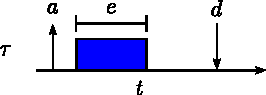
\includegraphics[width=0.50\linewidth]{fig/singleJob.pdf}
    \caption{Single Job Parameters} A single job of task $\tau$ with release time $a$, execution time $e$, and deadline $d$.
    \label{fig:rt-job}
\end{figure}

\subsubsection{Task}

A task, $\tau_i$, is an infinite series of jobs characterized by the tuple $\tau_i = (a,p,c,d)$ where $a$ is the offset of the task, $p$ is either the period or minimum interarrival, $c$ is the WCET, and $d$ is the relative deadline.
The offset, $a$, is the time after $t=0$ at which the first job of the task is released.
Tasks may be either aperiodic (also known as sporadic) or periodic.
Sporadic tasks release jobs at irregular intervals.
If $\tau$ is a sporadic task, $p$ represents the minimum interarrival time between successive jobs.
Periodic tasks release jobs at regular intervals.
If $\tau$ is a periodic task, $p$ represents the fixed interarrival time between successive jobs.
The WCET, $c$, is the upper bound on execution time for all jobs the task may release.
The relative deadline, $d$, is the relative deadline for all jobs of the task such that a job released at time $t$ is has a deadline at time $t+d$.
Figure \ref{fig:rt-task} illustrates a two tasks, one sporadic and one periodic, and their typical parameters.

\begin{figure}
    \centering
    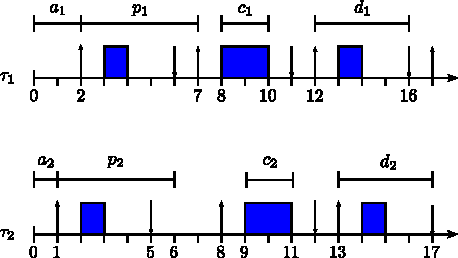
\includegraphics[width=0.75\linewidth]{fig/taskParameters.pdf}
    \caption{Task Parameters: Periodic and Sporadic} Task $\tau_1 = (a_1=2, p_1 = 5, c_1=2, d_1=4)$ is a periodic task.
    Task $\tau_2 = (a_2=1,p_2=5,c_2=2,d_2=4)$ is an aperiodic task.
    Note that $p_1$ is a period and each job of $\tau_1$ is released on a fixed interval.
    $p_2$ is a minimum interarrival time and each job of $\tau_2$ may have $p_2$ units of time or more between consecutive releases.
    \label{fig:rt-task}
\end{figure}

\subsubsection{Task Set}

When more than one task is needed to describe all computational loads, tasks are represented by a task set, $\Tau = \{\tau_1, \tau_2, \dots, \tau_n\}$, a collection of individual tasks.
From this task set, an additional parameter, the Hyperperiod $H$, can be derived.
The hyperperiod $H$ represents the least common multiple (LCM) of all periods (or minimum interarrival times) in  the task set.
Formally, $H = \text{LCM}(p_1, p_2, \dots, p_n)$.
This hyperperiod represents when pattern of computation repeats.

\subsection{Bounding Computation: Utilization and Demand}

With the fundamental tools for modeling computation described, we now describe tools to represent bounds on the total computation a task (or set of tasks) may require. 

\subsubsection{Utilization}

One method of bounding load is utilization, the ratio of WCET to period.
The utilization for an individual task is thus $u_i = \frac{c_i}{p_i}$.
The utilization for a task set is then,
\begin{equation}
    U = \sum_{i \in \Tau} \frac{c_i}{p_i}.
\end{equation}

Note that while utilization describes the ratio of time consumed to time available, it does not describe the change in computational load over time as jobs are released or job deadlines pass.

\subsubsection{Demand and the Demand Bound Function}

To provide a more precise bound on computation over time, demand is used.
The demand over some time interval $[t_1,t_2]$ is the sum of all WCETs of jobs with release time and deadline in the interval.
Demand, however, only reflects a particular interval and not any possible interval.
The Demand Bound Function (DBF), introduced by Baruah et al. \cite{baruah_preemptively_1990}, is a function which characterizes demand by providing the maximum cumulative execution time a set of tasks may require from a processor over any interval of size $\delta$. 
The definition presented in Baruah et al. \cite{baruah_preemptively_1990} is used here.
\begin{definition}[Demand bound Function]\label{def:dbf}
    The \textit{demand bound function}, $DBF(\tau,\delta)$, gives the cumulative WCET of all jobs of $\tau$ with both release times and deadlines within any time interval of length $\delta$.
\end{definition}

\subsection{Schedules, Feasibility, Scheduling Algorithms and Schedulability}

With utilization and the DBF to bound computation, we now introduce the schedule.

\subsubsection{Schedule}

A function describing which jobs or tasks are executed.
A map of workloads onto available time.

\subsubsection{Utilization}

\subsubsection{Demand Bound Function}


\subsubsection{Scheduling Algorithms}

An algorithm which takes tasks as inputs and generates a schedule.


